%
% quadratisch.tex -- 
%
% (c) 2021 Prof Dr Andreas Müller, OST Ostschweizer Fachhochschule
%
\documentclass[tikz]{standalone}
\usepackage{amsmath}
\usepackage{times}
\usepackage{txfonts}
\usepackage{pgfplots}
\usepackage{csvsimple}
\usetikzlibrary{arrows,intersections,math}
\begin{document}
\def\skala{1}
\begin{tikzpicture}[>=latex,thick,scale=\skala]

\node at (0,0) {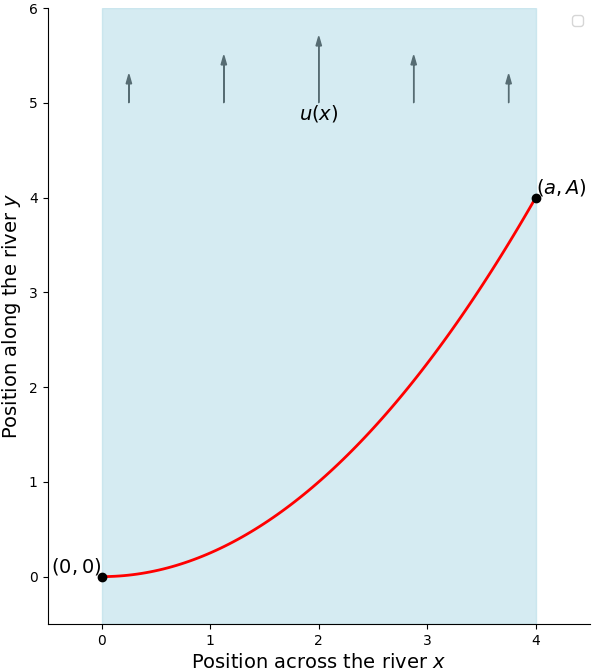
\includegraphics[width=7.56cm]{../Grafiken/Figure_1-crop.png}};
\fill[color=white] (3.35,3.8) rectangle ++(0.3,0.3);

\end{tikzpicture}
\end{document}

